\documentclass[11pt,a4paper]{article}
\usepackage[utf8]{inputenc}
\usepackage{amsmath,amssymb,amsfonts}
\usepackage{booktabs}
\usepackage{geometry}
\usepackage{hyperref}
\usepackage{caption}
\usepackage{threeparttable}
\usepackage{microtype}
\usepackage{graphicx}
\usepackage{comment}
\usepackage{xcolor}

% --- Packages ---
\usepackage[utf8]{inputenc}
\usepackage{amsmath, amssymb}
\usepackage[blocks]{authblk} % Handles multiple authors and affiliations cleanly
\usepackage{hyperref}


\graphicspath{{../paper_figures/}{outputs/paper_figures/}{../../outputs/paper_figures/}{images/}}

% --- Title & Metadata ---
\title{SUPPLEMENTARY MATERIAL\\[1ex]
\Large Critical Fragility Emerges from \\Chromosomal Instability in Cancer}
% --- Affiliation Definitions ---
\newcommand{\DFA}{Department of Physics and Astronomy ``Galileo Galilei'', University of Padova, Padova, Italy}
\newcommand{\CSL}{Complex Systems Lab, Universitat Pompeu Fabra, Dr Aiguader 88, 08003 Barcelona, Spain}
\newcommand{\CRG}{Centre de Regulaci\'{o} Gen\`{o}mica, Dr Aiguader 88, 003, Barcelona, Spain}
\newcommand{\CRM}{Centre de Recerca Matem\`{a}tica (CRM), Edifici C, Campus de Bellaterra 08193 Cerdanyola del Vall\`{e}s, Barcelona, Spain}
\newcommand{\ISEM}{ISEM, University Montpellier, CNRS, IRD, Montpellier, France}
\newcommand{\IBE}{Institut de Biologia Evolutiva, CSIC-UPF, Pg Maritim de la Barceloneta 37, 08003 Barcelona, Spain}
\newcommand{\ICREA}{Instituci\'{o} Catalana de la Recerca i Estudis Avan\c{c}ats, Psg Lluis Companys, Barcelona, Spain}
\newcommand{\SFI}{Santa Fe Institute, 1399 Hyde Park Road, Santa Fe NM 87501, USA}
\newcommand{\rev}[1]{\textcolor{blue}{#1}}

% --- Author Definitions ---
\author[1,2]{Francesco Zambelli}
\author[2]{Gianluca D'Addese}
\author[3]{Quim Marti Baena}
\author[4]{Josep Sardany\'{e}s}
\author[5]{Guim Aguad\'{e}-Gorgori\'{o}}
\author[2,6,7,8]{Ricard Sol\'{e}\thanks{Corresponding author: \texttt{ricard.sole@upf.edu}}}

% --- Affiliation Mapping ---
\affil[1]{\DFA}
\affil[2]{\CSL}
\affil[3]{\CRG}
\affil[4]{\CRM}
\affil[5]{\ISEM}
\affil[6]{\IBE}
\affil[7]{\ICREA}
\affil[8]{\SFI}


\begin{document}


\maketitle


\section{Agent-Based Model Specification: The ODD Protocol}
\label{sec:odd}

This section provides a standardized, comprehensive description of the \textbf{CancerEvo} individual-based simulation framework following the \textbf{ODD (Overview, Design concepts, Details) protocol} established by Grimm et al.\ (2006, 2010). The model simulates the stochastic eco-evolutionary dynamics of cancer cell populations under somatic point mutations, chromosomal instability, and spatial constraints, comparing a spatially structured solid tumor with a well-mixed liquid tumor.

\subsection{Overview}

\subsubsection{Purpose}
The primary purpose of the CancerEvo model is to investigate how the balance between selective growth advantages (oncogenes and tumor suppressor inactivation), mutator phenotypes (point mutation rate and chromosomal missegregation acceleration), and negative purifying selection (lethal homozygous inactivation of essential housekeeping genes) governs the evolutionary trajectories, clonal architecture, and non-equilibrium extinction thresholds of neoplasms. Specifically, the framework addresses:
\begin{enumerate}
    \item How spatial confinement in solid tissues (local competition within a Moore neighborhood on a 2D regular lattice) versus global fluid mixing in liquid malignancies (mean-field Moran competition) alters the critical mutation threshold separating viable tumor expansion from mutational meltdown (error catastrophe).
    \item How chromosomal instability (CIN) and segmental aneuploidy shape karyotypic fragility, buffering capacity, and the transition between diploid, polyploid, and aneuploid evolutionary equilibria.
    \item Whether therapeutically accelerating genomic instability can push tumors across the critical extinction boundary into an irreversible collapse phase.
\end{enumerate}

\subsubsection{Entities, State Variables, and Scales}
\paragraph{Individual Cells:} The primary active agents are individual biological cells occupying discrete sites within the tissue. Each cell $i$ is characterized by the following categorical and phenotypic state variables:
\begin{itemize}
    \item \textbf{Cellular State}: $\text{state}_i \in \{0, 1, 2\}$, where:
    \begin{itemize}
        \item $\text{state}_i = 0$: Healthy wild-type (WT) cell, dividing at homeostatic baseline rate $r_0$ with zero intrinsic mutation ($\mu_0 = 0$) and zero missegregation ($m_0 = 0$).
        \item $\text{state}_i = 1$: Cancer cell, possessing somatic driver mutations or karyotypic alterations, with evolving phenotypic rates $r_i$, $\mu_i$, and $m_i$.
        \item $\text{state}_i = 2$: Dead cell / vacant site. Generated when a cell suffers lethal mutational load or karyotypic nullisomy/overload ($r_i = 0, \mu_i = 0, m_i = 0$). A dead site exerts zero competitive resistance and is immediately available for colonization by dividing neighbors.
    \end{itemize}
    \item \textbf{Proliferation Rate}: $r_i \in [r_0, r_{\max}]$, representing the probability per unit time of attempting cell division. Wild-type cells divide at $r_0 = 0.15$, while cancer cells increase their proliferation rate in steps of $\Delta r = 0.008$ per activated driver, capped at $r_{\max} = 0.30$.
    \item \textbf{Point Mutation Rate}: $\mu_i \in [0, 1]$, the per-division probability of acquiring a point mutation at any present, unmutated gene locus. Cancer cells advance their mutation rate in increments of $\Delta\mu$ per inactivated mutator gene.
    \item \textbf{Missegregation Rate}: $m_i \in [0, 1]$, the probability per division of undergoing asymmetric chromosomal non-disjunction or segmental translocation, advancing in increments of $\Delta m$ per inactivated missegregation gene.
    \item \textbf{Ploidy (Chromosome Copy Number)}: $N_{\text{CHR}, i} \in \{1, 2, \dots, 5\}$, denoting the total number of physical chromosome homologues present in cell $i$. Cells are initialized as diploid ($N_{\text{CHR}} = 2$), except in designated haploid stability sweeps ($N_{\text{CHR}} = 1$). A cell experiencing nullisomy ($N_{\text{CHR}} = 0$) or karyotypic overload ($N_{\text{CHR}} > 5$) dies immediately.
\end{itemize}

\paragraph{Genomic Architecture and Locus Representation:}
Each chromosome copy $c \in \{1, \dots, N_{\text{CHR}}\}$ within cell $i$ contains $N_{\text{genes}} = 45$ functional gene loci, represented computationally by high-performance 64-bit integer bitmasks:
\begin{itemize}
    \item $\mathbf{C}_{c, i} \in \{0, 1\}^{N_{\text{genes}}}$ (\texttt{chromosomes}): Bitmask tracking somatic point mutations. A bit value of $0$ indicates an intact wild-type allele; a bit value of $1$ indicates a mutated allele.
    \item $\mathbf{P}_{c, i} \in \{0, 1\}^{N_{\text{genes}}}$ (\texttt{presence}): Bitmask tracking physical gene locus presence. A bit value of $1$ indicates that the locus is physically present on chromosome $c$; a bit value of $0$ indicates that the locus has been deleted (via segmental or whole-chromosome loss).
\end{itemize}
The 45 loci are partitioned into five functional classes:
\begin{enumerate}
    \item \textbf{Instability / Mutator Genes} ($N_I = 10$, bits 0--9): Recessive loci whose inactivation impairs DNA repair and increases the point mutation rate $\mu$.
    \item \textbf{Oncogenes} ($N_O = 10$, bits 10--19): Dominant driver loci whose mutational activation increases cellular proliferation rate $r$.
    \item \textbf{Tumor Suppressor Genes} ($N_S = 10$, bits 20--29): Recessive driver loci whose complete bi-allelic loss/inactivation increases cellular proliferation rate $r$.
    \item \textbf{Missegregation Genes} ($N_M = 5$, bits 30--34): Recessive loci whose inactivation impairs mitotic spindle checkpoints and increases chromosomal missegregation rate $m$.
    \item \textbf{Essential Housekeeping Genes} ($N_{HK} = 10$, bits 35--44): Strictly essential loci. Complete bi-allelic inactivation or deletion of any single housekeeping gene triggers deterministic cellular death.
\end{enumerate}

\paragraph{Spatial and Temporal Scales:}
\begin{itemize}
    \item \textbf{Solid Tumor Environment}: A two-dimensional regular square lattice of size $L \times L$ sites with rigid non-periodic boundaries ($N = L^2 = 6,400$ for bifurcation/phase diagrams, $N = 40,000$ for ensemble and intervention studies). Spatial interactions and competitive displacement occur within the local 8-cell Moore neighborhood (radius $R = 1$). A single lattice site represents the spatial footprint of one biological cell ($\sim 10\text{--}20\,\mu\text{m}$ in diameter), corresponding to a modeled tissue patch of $0.8 \times 0.8\,\text{mm}$ to $2.0 \times 2.0\,\text{mm}$.
    \item \textbf{Liquid Tumor Environment}: A non-spatial, well-mixed population of fixed carrying capacity $N = L^2$. Any dividing cell interacts globally with cells sampled uniformly at random across the entire tissue volume, representing circulating leukemias or ascites.
    \item \textbf{Temporal Scale}: Time progresses in discrete simulation steps $t = 1, 2, \dots, n_{\text{steps}}$ (up to $100,000$ steps for long-term critical slowing down investigations). Each step represents an epoch of stochastic division and replacement attempts scaled to cellular generation times.
\end{itemize}

\subsubsection{Process Overview and Scheduling}
Within each discrete simulation time step, the following processes occur sequentially:
\begin{enumerate}
    \item \textbf{Sampling of Reproducing Cells}: The total tissue proliferation potential $R = \sum_{i=1}^N r_i$ is evaluated. The number of division events $K$ occurring in the timestep is drawn from a Poisson distribution:
    \begin{equation}
        K \sim \text{Poisson}(R), \quad \text{with } K \le \sum_{i=1}^N \mathbb{I}(r_i > 0)
    \end{equation}
    A set of $K$ distinct mother cells is sampled without replacement with probabilities proportional to their division rates $w_i = r_i / R$.
    
    \item \textbf{Spatial Neighbor Selection and Competitive Replacement}:
    Each sampled mother cell $i$ attempts reproduction:
    \begin{itemize}
        \item \textit{Solid Model}: Cell $i$ inspects its Moore neighborhood $\mathcal{N}_i$. If cell $i$ is completely surrounded by healthy wild-type cells ($\text{state}_k = 0$ for all $k \in \mathcal{N}_i$), the division event is suppressed (simulating homeostatic contact inhibition). Otherwise, replacement is resolved in two hierarchical steps:
        \begin{enumerate}
            \item \textbf{Dead Site Colonization}: If dead cell sites ($\text{state} = 2$, $r = 0$) exist in $\mathcal{N}_i$, cell $i$ targets a vacant site with probability $n_{\text{dead}} / n_{\text{neigh}}$ and colonizes it deterministically ($P_{\text{replace}} = 1.0$).
            \item \textbf{Moran Contact Competition}: If no dead site is targeted, a living neighbor $j \in \mathcal{N}_i$ is selected uniformly at random. Cell $i$ displaces neighbor $j$ with symmetric Moran probability:
            \begin{equation}
                P_{\text{replace}}(i \to j) = \frac{r_i}{r_i + r_j}
            \end{equation}
            If the replacement check fails, the division attempt is aborted.
        \end{enumerate}
        \item \textit{Liquid Model}: A candidate target site $j$ is drawn uniformly from the entire population ($j \neq i$). If site $j$ is dead, replacement succeeds unconditionally. If site $j$ is living, replacement succeeds with Moran probability $r_i / (r_i + r_j)$.
    \end{itemize}
    
    \item \textbf{Clonal Replication and Daughter Placement}:
    Upon successful replacement, the mother cell remains at site $i$, while the newly generated daughter cell occupies target site $j$. The daughter initially inherits the exact karyotype, presence mask, and rates of the mother.
    
    \item \textbf{Point Mutation}:
    Both mother cell $i$ and daughter cell $j$ undergo independent somatic mutation. For every chromosome copy $c \in \{1, \dots, N_{\text{CHR}}\}$ and each locus $g \in \{0, \dots, N_{\text{genes}}-1\}$, if the locus is physically present ($\mathbf{P}_{c}[g] = 1$) and currently unmutated ($\mathbf{C}_{c}[g] = 0$), it mutates ($\mathbf{C}_{c}[g] \leftarrow 1$) with independent Bernoulli probability $\mu$.
    
    \item \textbf{Chromosomal Missegregation}:
    With probability $m_i$ (the mother's missegregation rate), an asymmetric segregation error occurs between mother $i$ and daughter $j$:
    \begin{itemize}
        \item \textit{Whole-Chromosome Mode (Polyploid / Numerical Aneuploidy)}: A chromosome copy is randomly selected from the mother and transferred to the daughter.
        \item \textit{Chunk Mode (Segmental Aneuploidy)}: A contiguous slice of loci of random length $\ell \in [3, N_{\text{genes}}-3]$ is deleted from one of the mother's homologues and appended to the daughter's lowest available chromosome slot.
    \end{itemize}
    The mother's chromosome array is compacted, and daughter chromosome slots are packed up to the maximum capacity of 6.
    
    \item \textbf{Phenotypic Rate Update}:
    The mutation rate $\mu$, division rate $r$, and missegregation rate $m$ of both mother and daughter are updated from their genomic bitmasks following the genotype-to-phenotype mapping rules (see Submodels).
    
    \item \textbf{Viability Check and Cell Death}:
    Both cells are evaluated for lethal genetic load. A cell suffers deterministic cell death if:
    \begin{itemize}
        \item Any essential housekeeping gene ($HK$) has lost all functional wild-type alleles (all copies mutated or deleted).
        \item The cell has suffered complete nullisomy ($N_{\text{CHR}} = 0$) or excessive karyotypic burden ($N_{\text{CHR}} > 5$).
    \end{itemize}
    Dying cells are converted to dead state ($\text{state} = 2, r = 0, \mu = 0, m = 0$), clearing their genomic bitmasks to create a vacant lattice site.
\end{enumerate}

\subsection{Design Concepts}

\paragraph{Basic Principles:}
The model integrates classical theoretical paradigms:
\begin{itemize}
    \item \textbf{Knudson's Two-Hit Hypothesis}: Tumor suppressor genes, mutator genes, missegregation genes, and housekeeping genes require bi-allelic (or multi-allelic under polyploidy) inactivation to manifest a phenotypic alteration.
    \item \textbf{Mutator Phenotype Hypothesis (Loeb)}: Somatic mutator mutations accelerate evolutionary search through driver fitness landscapes at the cost of escalating lethal mutational burden.
    \item \textbf{Error Catastrophe / Mutational Meltdown (Eigen)}: When the somatic mutation rate exceeds a critical threshold, negative selection acting on essential genes destroys clonal viability, driving the population into extinction.
    \item \textbf{Spatial Eco-Evolutionary Competition}: Contact inhibition and local Moran dynamics in solid tissues generate mechanical boundary effects absent in well-mixed regimes.
\end{itemize}

\paragraph{Emergence:}
Complex macro-scale behaviors emerge autonomously from local micro-scale interactions:
\begin{itemize}
    \item Spatial radial expansion, boundary-localized growth, and necrotic or quiescent cores.
    \item Clonal interference and hitchhiking of passenger mutations during selective sweeps.
    \item Non-equilibrium second-order phase transitions in solid tumors versus bistable first-order transitions in liquid tumors.
    \item Critical slowing down, characterized by variance divergence and autocorrelation peaking near the error catastrophe boundary.
    \item Emergent karyotype stabilization where aneuploid clones equilibrate around viable ploidies ($N_{\text{CHR}} = 2\text{--}3$) avoiding lethal housekeeping nullisomy.
\end{itemize}

\paragraph{Adaptation and Objective:}
Individual cells do not exhibit purposeful or cognitive adaptation. Cellular adaptation is strictly Darwinian: cells possessing mutations that confer elevated proliferation rates $r_i$ have an increased likelihood of being sampled for division and winning competitive replacement against neighbors, subject to surviving the housekeeping viability filter.

\paragraph{Sensing and Interaction:}
Dividing cells sense the physical presence (living vs.\ dead) and replication rates of their immediate Moore neighbors (in solid tumors) or globally sampled partners (in liquid tumors). Physical interactions are mediated entirely through space competition (displacing neighbors) and opportunistic colonization of vacant dead-cell sites.

\paragraph{Stochasticity:}
Stochasticity is explicitly modeled at all microscopic stages:
\begin{itemize}
    \item Poisson generation of total division counts per timestep.
    \item Fitness-weighted sampling of dividing cells without replacement.
    \item Uniform random selection of target neighbors within the Moore neighborhood.
    \item Moran acceptance probability for replacement events.
    \item Bernoulli trials for point mutations across present, unmutated loci.
    \item Random slice coordinates (start bit and length) during chunk missegregation.
    \item Stochastic spatial localization of initial tumor seed cells.
\end{itemize}

\paragraph{Collectives and Observation:}
Cells form clonal collectives sharing identical mutational profiles or karyotypes. At the population level, the model tracks global tumor density $f_C(t)$, dead cell density $f_{\text{dead}}(t)$, mean mutation rate $\langle \mu(t) \rangle$, mean division rate $\langle r(t) \rangle$, mean missegregation rate $\langle m(t) \rangle$, effective ploidy distributions $P(N_{\text{CHR}})$, locus-specific activation frequencies, and extinction times $T_{\text{ext}}$.

\subsection{Details}

\subsubsection{Initialization}
Simulations are initialized on a tissue grid of $L \times L$ sites (or global pool of size $N = L^2$):
\begin{itemize}
    \item \textbf{Background Healthy Tissue}: All $N$ sites are initialized as healthy wild-type cells ($\text{state} = 0, N_{\text{CHR}} = 2$). All 45 loci on both chromosome homologues are physically present ($\mathbf{P} = \text{mask\_all}$) and unmutated ($\mathbf{C} = 0$), yielding baseline division rate $r_{\text{WT}} = r_0 = 0.15$, mutation rate $\mu_0 = 0.0$, and missegregation rate $m_0 = 0.0$.
    \item \textbf{Cancer Seed Placement}:
    \begin{itemize}
        \item \textit{Solid Model}: Cancer seed cells are placed as a compact circular cluster centered at $(L/2, L/2)$ with radius $R_{\text{pert}} = r_{\text{pert}} \cdot L$. Default radius is $r_{\text{pert}} = 0.005$ ($\sim 5$ cells) for ensemble runs, $r_{\text{pert}} = 0.05$ ($\sim 314$ cells) for phase diagrams and interventions, and 10 cells for bifurcation runs (see Table~\ref{tab:simulation_configs}).
        \item \textit{Liquid Model}: Cancer seed cells ($n_{\text{seed}} = 10$ or $50$) are distributed uniformly at random across the tissue.
    \end{itemize}
    \item \textbf{Seed Genotype}: Seed cells are assigned homozygous mutations on both homologues at locus $I_1$ (bit 0) and locus $O_1$ (bit 10), with all other 43 loci unmutated. This immediately activates one instability gene ($k_I = 1 \implies \mu_{\text{seed}} = \mu_0 + \Delta\mu$) and one oncogene ($k_O = 1 \implies r_{\text{seed}} = r_0 + \Delta r$), establishing the founding malignant clone.
\end{itemize}

\subsubsection{Input Data}
The model is an autonomous, self-contained system and does not rely on exogenous environmental time-series data. In therapeutic intervention experiments, an external perturbation protocol is triggered dynamically when tumor density reaches $f_C(t) \ge 0.30$ (detailed in Section~\ref{sec:sim_params}, Table~\ref{tab:interventions}).

\subsubsection{Submodels}

\paragraph{Submodel 1: Genotype-to-Phenotype Mapping (Boolean Locus Logic)}
For cell $i$ with $N_{\text{CHR}}$ chromosomes, let $P_{c, g} \in \{0, 1\}$ and $C_{c, g} \in \{0, 1\}$ denote the presence and mutation status of locus $g \in \{0, \dots, N_{\text{genes}}-1\}$ on chromosome $c \in \{1, \dots, N_{\text{CHR}}\}$.
A locus possesses a functional wild-type allele if at least one chromosome copy carries a present, unmutated version:
\begin{equation}
    \text{FuncWT}(g) = \bigvee_{c=1}^{N_{\text{CHR}}} \left( P_{c, g} \land \neg C_{c, g} \right)
\end{equation}
Consequently, a recessive locus is completely inactivated if no chromosome carries a functional wild-type allele:
\begin{equation}
    \text{Inactivated}(g) = \neg \text{FuncWT}(g) = \bigwedge_{c=1}^{N_{\text{CHR}}} \left( \neg P_{c, g} \lor C_{c, g} \right)
\end{equation}
Active gene counts are computed according to biological dominance rules:
\begin{itemize}
    \item \textbf{Dominant Oncogenes} ($\mathcal{O}$, bits 10--19): An oncogene is activated if \emph{any} present copy is mutated:
    \begin{equation}
        k_O = \sum_{g \in \mathcal{O}} \bigvee_{c=1}^{N_{\text{CHR}}} \left( P_{c, g} \land C_{c, g} \right)
    \end{equation}
    \item \textbf{Recessive Tumor Suppressors} ($\mathcal{S}$, bits 20--29):
    \begin{equation}
        k_S = \sum_{g \in \mathcal{S}} \text{Inactivated}(g)
    \end{equation}
    \item \textbf{Recessive Instability / Mutator Genes} ($\mathcal{I}$, bits 0--9):
    \begin{equation}
        k_I = \sum_{g \in \mathcal{I}} \text{Inactivated}(g)
    \end{equation}
    \item \textbf{Recessive Missegregation Genes} ($\mathcal{M}$, bits 30--34):
    \begin{equation}
        k_M = \sum_{g \in \mathcal{M}} \text{Inactivated}(g)
    \end{equation}
\end{itemize}
Phenotypic rates are evaluated as:
\begin{equation}
    r_i = \min\left(r_{\max}, \; r_0 + (k_O + k_S) \cdot \Delta r\right), \quad \mu_i = \mu_0 + k_I \cdot \Delta\mu, \quad m_i = k_M \cdot \Delta m
\end{equation}
where baseline parameters ($r_0, \Delta r, r_{\max}, \mu_0$) are listed in Table~\ref{tab:baseline_params}.

\paragraph{Submodel 2: Lethal Mutational Load and Cell Death}
Cell death is evaluated deterministically. A cell is non-viable and converted to dead state ($\text{state}_i \leftarrow 2$) if it satisfies any of the following biological lethality criteria:
\begin{equation}
    \left[ \exists g \in \mathcal{HK} \quad \text{such that} \quad \text{Inactivated}(g) = 1 \right] \quad \lor \quad N_{\text{CHR}, i} = 0 \quad \lor \quad N_{\text{CHR}, i} > 5
\end{equation}

\subparagraph{Application to Aneuploid and Heteroploid Cells:}
The presence-aware Boolean logic ($\text{Inactivated}(g) = \bigwedge_{c} [\neg P_{c,g} \lor C_{c,g}]$) governs cell fate across numerical and segmental aneuploidy in three distinct operational regimes:
\begin{enumerate}
    \item \textbf{Locus Nullisomy (Segmental or Whole-Chromosome Loss)}: If a cell loses an allele of housekeeping gene $g$ through chunk deletion or chromosome loss, the locus becomes hemizygous ($P_{c,g} = 1$ on only one homologue). If that remaining copy is subsequent deleted ($\forall c, P_{c,g} = 0$), the locus suffers physical nullisomy, immediately rendering $\text{Inactivated}(g) = 1$ and triggering instantaneous cell death.
    \item \textbf{Hemizygous Vulnerability}: In a cell that is hemizygous for housekeeping gene $g$ (due to prior segmental deletion or monosomy, $N_{\text{CHR}} = 1$), a single somatic point mutation on the lone surviving allele ($C_{1,g} \leftarrow 1$) eliminates the only functional copy ($\text{FuncWT}(g) = 0$), causing cell death. In contrast to diploid cells (which require two hits), hemizygous clones possess zero buffering capacity.
    \item \textbf{Polyploid Buffering and Cryptic Damage}: In polysomic or polyploid cells ($N_{\text{CHR}} \in \{3, 4, 5\}$), a housekeeping locus remains functional as long as at least one intact copy survives. These cells can accumulate deleterious mutations on multiple copies without dying (buffering capacity). However, if subsequent missegregation transfers away or deletes the single remaining functional copy, the cell is left exclusively with mutated alleles, triggering delayed catastrophic collapse (karyotypic fragility).
    \item \textbf{Global Ploidy Bounds}: A cell dies immediately if it suffers total chromosome loss ($N_{\text{CHR}} = 0$, complete nullisomy) or exceeds the maximum viable karyotype limit ($N_{\text{CHR}} > 5$, representing proteotoxic stress and severe mitotic catastrophe).
\end{enumerate}
Crucially, lethality is evaluated twice within every division event: first immediately following point mutation, and re-evaluated immediately following chromosome/chunk transfer for both mother and daughter cells. If a transfer deprives the mother of its last functional housekeeping allele or pushes the daughter's ploidy beyond 5, that cell is converted to dead site ($\text{state} = 2, r = 0, \mu = 0, m = 0$), clearing all genomic arrays.

\paragraph{Submodel 3: Moran Competition and Replacement Dynamics}
When dividing mother cell $i$ targets neighbor site $j$:
\begin{equation}
    P_{\text{replace}}(i \to j) = 
    \begin{cases}
        1.0, & \text{if site } j \text{ is dead } (\text{state}_j = 2, r_j = 0) \\[4pt]
        \dfrac{r_i}{r_i + r_j}, & \text{if site } j \text{ is living } (\text{state}_j \in \{0, 1\})
    \end{cases}
\end{equation}
In the solid model, if dead neighbors exist in the Moore neighborhood $\mathcal{N}_i$, dead sites are targeted with probability $n_{\text{dead}} / n_{\text{neigh}}$ to prioritize filling tissue voids before displacing living neighbors.

\paragraph{Submodel 4: Chromosomal Missegregation Mechanics}
When missegregation occurs (with probability $m_i$):
\begin{itemize}
    \item \textbf{Whole-Chromosome Transfer}: A random chromosome $c_{\text{donor}} \in \{1, \dots, N_{\text{CHR}, i}\}$ is selected from mother $i$. The full chromosome (mutations and presence masks) is removed from mother $i$ and transferred into the lowest unoccupied slot of daughter $j$.
    \item \textbf{Chunk-Based Segmental Missegregation}: A cut length $\ell \in \{3, \dots, N_{\text{genes}}-3\}$ and start locus $g_{\text{start}} \in \{0, \dots, N_{\text{genes}}-1\}$ are chosen uniformly at random. A contiguous bitwise mask of length $\ell$ with periodic wrap-around is defined:
    \begin{equation}
        \mathbf{M}_{\text{chunk}} = \bigvee_{b=0}^{\ell-1} \left( 1 \ll \left[ (g_{\text{start}} + b) \pmod{N_{\text{genes}}} \right] \right)
    \end{equation}
    The slice $\mathbf{S} = \mathbf{M}_{\text{chunk}} \land \mathbf{P}_{c_{\text{donor}}, i}$ is removed from the mother's homologue ($\mathbf{P}_{c_{\text{donor}}, i} \leftarrow \mathbf{P}_{c_{\text{donor}}, i} \land \neg\mathbf{S}$, $\mathbf{C}_{c_{\text{donor}}, i} \leftarrow \mathbf{C}_{c_{\text{donor}}, i} \land \neg\mathbf{S}$) and integrated into the daughter cell across available slots $c \in \{1, \dots, 6\}$.
\end{itemize}
Following transfer, the mother cell compacts its remaining chromosome slots, and both mother and daughter re-evaluate their viability and phenotypic rates.

\clearpage

\section{Analytical Master Equation and Stationary Mutational Distributions in Liquid Tumors}
\label{sec:analytical}

We consider a liquid tumor model with fixed population size $N$. The number of wild-type cells is indicated with $W$, the number of dead cells with $D$. The cancer cell population can be further divided in $N_{\mathcal{I}}$ sub-populations (one per instability class), with $N_{\mathcal{I}}$ the number of instability genes. We indicate the abundance of each cancer sub-population with $C_k$, where $k \in \{1, \dots, N_I\}$ counts the number of mutated instability genes. We work with densities (fractions) rather than absolute abundances:

\begin{equation}
    f_W \equiv \frac{W}{N}, \quad f_k \equiv \frac{C_k}{N}, \quad p_D \equiv \frac{D}{N}
\end{equation}

These are constrained by the fixed-size normalization:
\begin{equation}
    \sum_{k=1}^{N_I} f_k + f_W + p_D = 1
\end{equation}

\subsubsection*{Survival probability after a mutation round}

Both cancer and wild-type cells undergo replication followed by a stochastic mutation event. After mutation, a viability check is performed on all $N_{HK}$ housekeeping genes: if any housekeeping gene becomes fully mutated (on all chromosome copies), the cell dies. Each gene has an independent per-locus mutation probability $\mu_k = k \cdot \delta\mu$ for a class-$k$ cell. The probability that a single housekeeping gene survives (i.e.\ is not mutated) in one round is $(1 - k\,\delta\mu)$. Since all $N_{HK}$ housekeeping genes must independently survive:

\begin{equation}
    P_{s,k} = \underbrace{(1 - k\,\delta\mu)}_{\text{one HK gene survives}} \times \cdots \times \underbrace{(1 - k\,\delta\mu)}_{N_{HK}\text{ times}} = (1 - k\,\delta\mu)^{N_{HK}}
\end{equation}

\subsubsection*{The post-replication fates (exact multi-step model)}

After a mutation round, a cell in class $k$ can either remain in class $k$ (cloning), promote to class $k+j$ with $j \ge 1$ (multi-step promotion), or die due to a housekeeping mutation. Since mutations at different loci occur independently with per-locus probability $\mu_k = k \cdot \delta\mu$, we derive these probabilities exactly:

\paragraph{1. Faithful cloning ($\alpha_k$):} The cell remains in class $k$. This requires that none of the $N_{HK}$ housekeeping genes and none of the $(N_I - k)$ remaining unmutated instability genes are hit. The total number of loci that must remain unmutated is $N_{HK} + N_I - k$:
\begin{equation}
    \alpha_k = (1 - k\,\delta\mu)^{N_{HK} + N_I - k}
\end{equation}

\paragraph{2. Promotion ($P_{k \to k+j}$):} The cell advances from class $k$ to class $k+j$ (where $j \in \{1, \dots, N_I - k\}$ instability genes mutate, while all other instability loci and all housekeeping loci remain unmutated). Since the selection of which instability genes mutate is combinatorial:
\begin{equation}
    P_{k \to k+j} = \binom{N_I - k}{j} (k\,\delta\mu)^j (1 - k\,\delta\mu)^{N_{HK} + N_I - k - j}
\end{equation}
Note that faithful cloning is simply the diagonal case $\alpha_k = P_{k \to k}$.

\paragraph{3. Lethal mutation ($\delta_k$):} The cell dies because at least one housekeeping gene is hit, which is the complement of the survival probability $P_{s,k} = (1 - k\,\delta\mu)^{N_{HK}}$:
\begin{equation}
    \delta_k = 1 - P_{s,k} = 1 - (1 - k\,\delta\mu)^{N_{HK}}
\end{equation}

The sum of all possible survival outcomes plus the death probability is exactly 1:
\begin{equation}
    \sum_{j=0}^{N_I - k} P_{k \to k+j} + \delta_k = (1 - k\,\delta\mu)^{N_{HK}} \sum_{j=0}^{N_I - k} \binom{N_I - k}{j} (k\,\delta\mu)^j (1 - k\,\delta\mu)^{N_I - k - j} + [1 - (1 - k\,\delta\mu)^{N_{HK}}] = 1
\end{equation}

This binomial formulation provides an exact description of the mutation process without needing leading-order approximations.

\subsubsection*{Moran competition probabilities}

When a dividing cell targets a living (non-dead) cell, the outcome is decided by a Moran process: the divider replaces the target with probability proportional to its fitness relative to the combined fitness. All cancer classes share the same intrinsic division rate $r_m$, while wild-type cells divide at rate $r_0$:

\begin{itemize}
    \item \textbf{Cancer vs Wild-Type:} The cancer cell (rate $r_m$) competes against a wild-type cell (rate $r_0$):
    \begin{equation}
        \beta_{cw} = \frac{r_m}{r_m + r_0}
    \end{equation}
    \item \textbf{Cancer vs Cancer:} Two cancer cells with the same rate $r_m$ compete symmetrically:
    \begin{equation}
        \beta_{cc} = \frac{r_m}{r_m + r_m} = \frac{1}{2}
    \end{equation}
    \item \textbf{Wild-Type vs Cancer:} The complement of the cancer-vs-WT outcome:
    \begin{equation}
        \beta_{wc} = \frac{r_0}{r_m + r_0} = 1 - \beta_{cw}
    \end{equation}
\end{itemize}

System parameters are formalized in Table~\ref{tab:parameters}.

\begin{table}[htbp]
\centering
\caption{Systematic Overview of the Unified Parameter Space}
\label{tab:parameters}
\begin{tabular}{lll}
\toprule
\textbf{Symbol} & \textbf{Biological Definition} & \textbf{Functional Form / Constraint} \\
\midrule
$N$ & Total fixed tissue lattice sites & Constant volume constraint \\
$N_I$ & Maximum viable cancer mutational classes & Total mutable Instability genes \\
$N_{HK}$ & Total critical Housekeeping genes & Continuous fitness check loci \\
$\delta\mu$ & Per-locus mutation rate increment & Constant scaling factor \\
$r_m$ & Intrinsic division rate of class $k$ cancer & Phenotypic fitness parameter \\
$r_0$ & Active division rate of healthy wild-type & Homeostatic driver baseline \\
$\alpha_k$ & Probability of a faithful clone & $(1-k\,\delta\mu)^{N_{HK} + N_I - k}$ \\
$P_{k \to k+j}$ & Probability of promotion ($k \to k+j$) & $\binom{N_I-k}{j}(k\,\delta\mu)^j(1-k\,\delta\mu)^{N_{HK}+N_I-k-j}$ \\
$\delta_k$ & Lethal mutation probability & $1 - (1-k\,\delta\mu)^{N_{HK}}$ \\
$\beta_{cw}$ & Moran win probability of cancer vs WT & $r_m / (r_m + r_0)$ \\
$\beta_{cc}$ & Moran win probability of cancer $k$ vs $j$ & $r_m / (r_m + r_m)$ \\
$\beta_{wc}$ & Moran win probability of WT vs cancer $k$ & $r_0 / (r_m + r_0) = 1 - \beta_{cw}$ \\
\bottomrule
\end{tabular}
\end{table}

\subsection{Microscopic Mechanisms and Elementary Transition Rates}

After each duplication step, both mother and daughter cells independently undergo stochastic mutation events as described above. Both cells independently draw from the same probability distribution: cloning ($\alpha_k$), promoting ($P_{k \to k+j}$), or dying ($\delta_k$). Crucially, DNA replication and subsequent viability/mutation checks are only performed upon successful division (Moran competition success). If division is aborted, neither the mother nor the daughter replicates or mutates. Thus, all division-dependent rates (cloning, promotion, and death) for both mother and daughter cells are scaled by the division success probability $\phi_k$.

\subsubsection*{Effective reachable space $\phi_k$}

We define the fractional reachable space $\phi_k$ as the effective probability that a dividing class-$k$ cancer cell successfully places its daughter. The daughter can land on three types of targets:

\begin{equation}
    \phi_k = \underbrace{p_D}_{\substack{\text{dead slots:}\\\text{always available}}}
           + \underbrace{f_W\,\beta_{cw}}_{\substack{\text{WT cells displaced}\\\text{via Moran competition}}}
           + \underbrace{\sum_{j=1}^{N_I} f_j\,\beta_{cc}}_{\substack{\text{cancer cells displaced}\\\text{(50\% win rate)}}}
\end{equation}

\begin{itemize}
    \item $p_D$: the fraction of dead (empty) slots. Replacement always succeeds (no competition needed).
    \item $f_W \beta_{cw}$: wild-type cells are encountered with frequency $f_W$, and the cancer cell wins the Moran competition with probability $\beta_{cw}$.
    \item $\sum_j f_j \beta_{cc}$: other cancer cells are encountered with total frequency $\sum_j f_j$, with a symmetric 50\% win rate $\beta_{cc} = 1/2$.
\end{itemize}

\subsubsection*{Elementary transitions}

We now enumerate every possible microscopic event and its rate. The key insight is that during a single division event of a class-$k$ cancer cell, two independent fates are resolved: (i) the \textbf{mother fate} (what happens to the original cell on its site after mutation), and (ii) the \textbf{daughter fate} (what happens to the copy placed at the target site after mutation). Both fates are conditioned on the division being successfully completed.

The complete transition rate matrix is given in Table~\ref{tab:transitions}. We explain each row below.

\begin{table}[htbp]
\centering
\caption{Complete Microscopic Transition Rate Matrix (Symmetrical Hazards)}
\label{tab:transitions}
\resizebox{\textwidth}{!}{% 
\begin{tabular}{lllll}
\toprule
\textbf{Active Vector} & \textbf{Target \& Event Type} & $\mathbf{\Delta C_k}$ & $\mathbf{\Delta D}$ & \textbf{Transition Rate ($\lambda$)} \\
\midrule
Cancer Class $k$ & \textbf{Mother Fate:} Dies on Site & $-1$ & $+1$ & $C_k \, r_m \, \phi_k \, \delta_k$ \\
Cancer Class $k$ & \textbf{Mother Fate:} Promotes on Site ($k \to k+j$) & $-1_{k}, +1_{k+j}$ & $0$ & $C_k \, r_m \, \phi_k \, P_{k \to k+j}$ \\
Cancer Class $k$ & \textbf{Daughter Fate:} Clones on $D$ & $+1$ & $-1$ & $C_k \, r_m \, p_D \, \alpha_k$ \\
Cancer Class $k$ & \textbf{Daughter Fate:} Promotes on $D$ ($k \to k+j$) & $+1_{k+j}$ & $-1$ & $C_k \, r_m \, p_D \, P_{k \to k+j}$ \\
Cancer Class $k$ & \textbf{Daughter Fate:} Dies on $D$ & $0$ & $0$ & $C_k \, r_m \, p_D \, \delta_k$ \\
Cancer Class $k$ & \textbf{Daughter Fate:} Clones on $W$ & $+1$ & $0$ & $C_k \, r_m \, f_W \, \beta_{cw} \, \alpha_k$ \\
Cancer Class $k$ & \textbf{Daughter Fate:} Dies on $W$ & $0$ & $+1$ & $C_k \, r_m \, f_W \, \beta_{cw} \, \delta_k$ \\
Wild-Type ($W$) & WT Divides, Replaces Dead Void & $0$ & $-1$ & $W \, r_0 \, p_D$ \\
Wild-Type ($W$) & WT Divides, Clears Cancer $k$ & $-1$ & $0$ & $W \, r_0 \, f_k \, \beta_{wc}$ \\
\bottomrule
\end{tabular}%
} % 
\end{table}

\begin{comment}
    \paragraph{Explanation of each transition rate:}
\begin{enumerate}
    \item \textbf{Mother dies on site} ($C_k\, r_m\, \phi_k\, \delta_k$): A class-$k$ cell successfully initiates division (probability $\phi_k$), and the mother undergoes a lethal housekeeping mutation (probability $\delta_k$). The cell dies in place: $C_k \to C_k - 1$, $D \to D + 1$.

    \item \textbf{Mother promotes on site} ($C_k\, r_m\, \phi_k\, P_{k \to k+j}$): The mother successfully initiates division and mutates $j$ instability genes, advancing to class $k+j$ \emph{without leaving its site}. This is a type-swap: $C_k \to C_k - 1$, $C_{k+j} \to C_{k+j} + 1$, with no change to $D$.

    \item \textbf{Daughter clones on dead slot} ($C_k\, r_m\, p_D\, \alpha_k$): The daughter targets a dead slot (probability $p_D$) and faithfully clones (probability $\alpha_k$). Net effect: $C_k \to C_k + 1$, $D \to D - 1$.

    \item \textbf{Daughter promotes on dead slot} ($C_k\, r_m\, p_D\, P_{k \to k+j}$): The daughter targets a dead slot and mutates $j$ instability genes during division. Net effect: $C_{k+j} \to C_{k+j} + 1$, $D \to D - 1$.

    \item \textbf{Daughter dies on dead slot} ($C_k\, r_m\, p_D\, \delta_k$): The daughter targets a dead slot but suffers a lethal mutation. The dead slot remains dead, and no net population change occurs ($\Delta C_k = 0$, $\Delta D = 0$).

    \item \textbf{Daughter clones on WT} ($C_k\, r_m\, f_W\, \beta_{cw}\, \alpha_k$): The daughter targets a wild-type cell (probability $f_W$), wins the Moran competition (probability $\beta_{cw}$), and faithfully clones ($\alpha_k$). The WT cell is displaced: $C_k \to C_k + 1$, $W \to W - 1$.

    \item \textbf{Daughter dies on WT} ($C_k\, r_m\, f_W\, \beta_{cw}\, \delta_k$): The daughter wins competition against a WT cell but then suffers a lethal mutation. The WT cell is lost and a dead cell appears: $D \to D + 1$, $W \to W - 1$.

    \item \textbf{WT replaces dead slot} ($W\, r_0\, p_D$): A wild-type cell divides (rate $r_0$) and fills a dead slot (probability $p_D$). Net: $W \to W + 1$, $D \to D - 1$. No Moran competition is needed against dead cells.

    \item \textbf{WT clears cancer} ($W\, r_0\, f_k\, \beta_{wc}$): A wild-type cell targets a class-$k$ cancer cell (probability $f_k$) and wins the Moran competition with probability $\beta_{wc}$. Net: $C_k \to C_k - 1$, $W \to W + 1$.
\end{enumerate}
\end{comment}


\subsection{Mean-Field Ordinary Differential Equations}

By taking the thermodynamic limit ($N \to \infty$), the stochastic master equation converges to a deterministic system of ODEs. We derive the ODE for each compartment by summing all transition rates from Table~\ref{tab:transitions} that affect that compartment, converting from absolute counts to densities ($f_k = C_k/N$).

\subsubsection*{Interior cancer classes ($1 < k < N_I$)}

For an interior cancer class $k$ ($1 < k < N_I$), the rate of change of the cell fraction $f_k$ is determined by five primary biological processes: (i) net clonal growth and survival ($r_m f_k \phi_k (2\alpha_k - 1)$), which balances faithful daughter cloning against mother cell loss via death or promotion; (ii) self-displacement loss within the same class ($r_m f_k^2 / 2$); (iii) cross-class loss due to displacement by other cancer classes ($f_k \sum_{j \neq k} r_m f_j \beta_{cc}$); (iv) wild-type clearance loss ($r_0 f_W f_k \beta_{wc}$); and (v) promotion influx from all upstream classes $i < k$ ($\sum_{i=1}^{k-1} 2\, r_m f_i \phi_i P_{i \to k}$). Combining these contributions yields:
\begin{equation}
    \frac{df_k}{dt} = r_m f_k \phi_k (2\alpha_k - 1)
    - r_m \frac{f_k^2}{2}
    - f_k \!\sum_{j \neq k}\! r_m f_j \beta_{cc}
    - r_0 f_W f_k \beta_{wc}
    + \sum_{i=1}^{k-1} 2\, r_m f_i \phi_i P_{i \to k}
\end{equation}

\subsubsection*{Boundary class $k = 1$}

The founding cancer class $k=1$ receives no upstream mutational influx (there is no class $k=0$). The equation is identical to the interior case but without Term~6:
\begin{equation}
    \frac{df_1}{dt} = r_m f_1 \phi_1 (2\alpha_1 - 1) - r_m \frac{f_1^2}{2} - f_1 \sum_{j \neq 1} r_m f_j \beta_{cc} - r_0 f_W f_1 \beta_{wc}
\end{equation}

\subsubsection*{Terminal class $k = N_I$}

For the terminal mutational class, all instability genes are already mutated, so further promotion is impossible: $P_{N_I \to N_I+j} = 0$. The mother-loss term simplifies to $-r_m f_{N_I} \phi_{N_I} (1 - \alpha_{N_I})$ where $1 - \alpha_{N_I} = \delta_{N_I}$. The promotion influx from all classes $i < N_I$ is present:
\begin{equation}
    \frac{df_{N_I}}{dt} = r_m f_{N_I} \phi_{N_I} (2\alpha_{N_I} - 1) - r_m \frac{f_{N_I}^2}{2} - f_{N_I} \sum_{j \neq N_I} r_m f_j \beta_{cc} - r_0 f_W f_{N_I} \beta_{wc} + \sum_{i=1}^{N_I-1} 2\, r_m f_i \phi_i P_{i \to N_I}
\end{equation}

\subsubsection*{Wild-type compartment $f_W$}

The WT population grows when WT cells divide and successfully place daughters on dead slots or displace cancer cells, and shrinks when cancer daughters displace WT cells:

\begin{itemize}
    \item \textbf{Gain:} WT divides onto dead slots (rate $r_0 f_W p_D$) or displaces cancer class $j$ (rate $r_0 f_W f_j \beta_{wc}$ per class).
    \item \textbf{Loss:} Cancer class $k$ daughters displace WT cells (rate $r_m f_k f_W \beta_{cw}$ per class).
\end{itemize}

\begin{equation}
    \frac{df_W}{dt} = \underbrace{r_0 f_W \left( p_D + \sum_{j=1}^{N_I} f_j \beta_{wc} \right)}_{\text{WT expansion (dead slots + cancer clearance)}} - \underbrace{f_W \sum_{k=1}^{N_I} r_m f_k \beta_{cw}}_{\text{displacement by cancer daughters}}
\end{equation}

\subsubsection*{Dead compartment $p_D$}

Dead cells accumulate from lethal mutations (both mother dying in place and daughter dying after placement) and are consumed when any living cell fills a dead slot. Since DNA replication only happens during successful division, both mother and daughter can only die if division succeeds.

\begin{itemize}
    \item \textbf{Gain from mother death:} $r_m f_k \phi_k \delta_k$ per class (row 1).
    \item \textbf{Gain from daughter death:} $r_m f_k \phi_k \delta_k$ per class (combining rows 5, 7, and cancer-cancer targets).
    \item \textbf{Total death-related gain:} $2\, r_m f_k \phi_k \delta_k$ per class.
    \item \textbf{Loss from filling:} Dead slots are consumed by cancer daughters ($r_m f_k p_D$, regardless of fate) and WT daughters ($r_0 f_W p_D$).
\end{itemize}

\begin{equation}
    \frac{dp_D}{dt} = \underbrace{\sum_{k=1}^{N_I} r_m f_k \left[ 2 \phi_k \delta_k - p_D \right]}_{\text{cancer-driven death accumulation minus filling}} - \underbrace{r_0 f_W p_D}_{\text{WT filling dead slots}}
\end{equation}

\subsection{Stationary State Distributions and Stability Analysis}

\subsubsection*{Linear stability of the healthy fixed point}

We examine the linear stability of the healthy fixed point $(f_W^* = 1,\; p_D^* = 0,\; f_k^* = 0\;\forall k)$ against an infinitesimal perturbation $f_1 = \epsilon \ll 1$, with all other cancer classes still at zero.

Starting from the $k=1$ boundary ODE and substituting the healthy fixed-point values, each term simplifies as follows:

\begin{itemize}
    \item \textbf{Mother loss \& daughter clone (combined):} $r_m\,\epsilon\,\phi_1\,(2\alpha_1 - 1)$. At the fixed point, $\phi_1 \to f_W \beta_{cw} = 1 \cdot \beta_{cw}$. This gives $r_m\,\beta_{cw}\,(2\alpha_1 - 1)\,\epsilon$.
    \item \textbf{Self-displacement:} $-r_m\,\epsilon^2/2 \approx 0$ --- vanishes at $\mathcal{O}(\epsilon^2)$.
    \item \textbf{Cross-class loss:} $-\epsilon \sum_{j\neq 1} r_m f_j \beta_{cc} = 0$.
    \item \textbf{WT clearance:} $-r_0\,(1)\,\epsilon\,\beta_{wc} = -r_0\,\beta_{wc}\,\epsilon$.
    \item \textbf{Promotion influx:} absent for $k=1$.
\end{itemize}

Collecting all $\mathcal{O}(\epsilon)$ terms:
\begin{equation}
    \frac{df_1}{dt} \approx \left[ r_m\,\beta_{cw}\,(2\alpha_1 - 1) - r_0\,\beta_{wc} \right] \epsilon
\end{equation}

Substituting $\beta_{cw} = r_m/(r_m + r_0)$ and $\beta_{wc} = r_0/(r_m + r_0)$:
\begin{equation}
    \frac{df_1}{dt} \approx \rev{\frac{r_m^2\,(2\alpha_1 - 1) - r_0^2}{r_m + r_0}} \, f_1
\end{equation}

\subsubsection*{Derivation of the growth foothold inequality}

The tumor can invade when the bracketed growth rate is positive:
\begin{equation}
    \rev{r_m^2\,(2\alpha_1 - 1) - r_0^2 > 0}
\end{equation}

This yields the Unified Growth Foothold Inequality:
\begin{equation}
    \rev{r_m^2\,(2\alpha_1 - 1) > r_0^2 \iff 2\alpha_1 - 1 > \left(\frac{r_0}{r_m}\right)^{\!2} \iff \alpha_1 > \frac{1 + (r_0/r_m)^2}{2}}
\end{equation}

The left-hand side balances the cancer cell's maximum birth rate times its net clonal expansion factor $(2\alpha_1 - 1)$, which accounts for the survival and fidelity of both the mother and daughter during a division event. The right-hand side $r_0$ represents the WT homeostatic division pressure. When mutation rates are too high, the cancer's net growth rate drops below the wild-type's division rate, preventing the tumor from taking foothold. \rev{The quadratic scaling in $r_m^2$ and $r_0^2$ emerges because replacement requires both division and competitive Moran displacement, so each cell type's effective expansion power scales with the square of its proliferation rate.}

\subsubsection*{Stationary state}

When the growth inequality is satisfied, the system reaches a tumor-dominated stationary state where $df_k/dt = 0$ for all $k$. Setting the interior ODE to zero and rearranging:

\begin{equation}
    0 = r_m f_k^* \phi_k^* (2\alpha_k - 1) - r_m \frac{(f_k^*)^2}{2} - f_k^* \sum_{j \neq k} r_m f_j^* \beta_{cc} - r_0 f_W^* f_k^* \beta_{wc} + \sum_{i=1}^{k-1} 2\, r_m f_i^* \phi_i^* P_{i \to k}
\end{equation}

We separate the $\phi_k^*$ sum into its self-interaction part ($f_k^* \beta_{cc}$) and the rest ($\phi_k^{(\neq k)*}$):
\begin{equation}
    \phi_k^* = \phi_k^{(\neq k)*} + f_k^*\,\beta_{cc}
\end{equation}

Substituting and grouping terms by powers of $f_k^*$:

\begin{align}
    0 &= r_m f_k^* \left[\phi_k^{(\neq k)*} + f_k^* \beta_{cc}\right] (2\alpha_k - 1) - r_m \frac{(f_k^*)^2}{2} \nonumber \\
      &\quad - f_k^* \sum_{j \neq k} r_m f_j^* \beta_{cc} - r_0 f_W^* f_k^* \beta_{wc} + \sum_{i=1}^{k-1} 2\, r_m f_i^* \phi_i^* P_{i \to k} \nonumber \\
    0 &= r_m f_k^* \phi_k^{(\neq k)*} (2\alpha_k - 1) + r_m (f_k^*)^2 \beta_{cc} (2\alpha_k - 1) - r_m \frac{(f_k^*)^2}{2} \nonumber \\
      &\quad - f_k^* \sum_{j \neq k} r_m f_j^* \beta_{cc} - r_0 f_W^* f_k^* \beta_{wc} + \sum_{i=1}^{k-1} 2\, r_m f_i^* \phi_i^* P_{i \to k}
\end{align}

Since $\beta_{cc} = 1/2$, the quadratic terms combine as:
\begin{equation}
    -r_m (1 - \alpha_k) (f_k^*)^2
\end{equation}

Collecting terms, this takes the standard quadratic form:

\begin{equation}
    A_k\,(f_k^*)^2 - B_k\,f_k^* - Q_{k-1}^* = 0
\end{equation}

where the coefficients are:

\begin{enumerate}
    \item \textbf{Quadratic (self-interaction) coefficient ($A_k$):}
    
\begin{equation}
    A_k = r_m (1 - \alpha_k)
\end{equation}

This arises from the combination of self-displacement ($\beta_{cc} = 1/2$) and the mutation outcomes.

\item \textbf{Linear (net growth) coefficient ($B_k$):}
\begin{equation}
    B_k = r_m\,\phi_k^{(\neq k)*}\,(2\alpha_k - 1) - \sum_{j \neq k} r_m f_j^*\,\beta_{cc} - r_0\,f_W^*\,\beta_{wc}
\end{equation}
This coefficient represents the net per-capita growth rate of class $k$ at the stationary state, excluding self-interaction and upstream promotion.
\item \textbf{Upstream promotion source ($Q_{k-1}^*$):}
\begin{equation}
    Q_{k-1}^* = \sum_{i=1}^{k-1} 2\, r_m\,f_i^*\,\phi_i^*\,P_{i \to k}
\end{equation}
This is the rate at which cells flow into class $k$ from all lower classes $i < k$ (dual-sourced: mother promoting + daughter promoting). For $k=1$, $Q_0^* = 0$.
\end{enumerate}

\subsubsection*{Solution via the quadratic formula}

The quadratic $A_k x^2 - B_k x - Q_{k-1}^* = 0$ (with $x = f_k^*$) has the physical (positive) root:
\begin{equation}
    f_k^* = \frac{B_k + \sqrt{B_k^2 + 4\,A_k\,Q_{k-1}^*}}{2\,A_k}
    \label{eq:sta_distr}
\end{equation}

The positive sign before the square root is chosen because $f_k^* \geq 0$ is required. The system is solved sequentially: $f_1^*$ is determined first (with $Q_0^* = 0$), then $f_2^*$ using $f_1^*$, and so on up to $f_{N_I}^*$.

\section{Simulation Parameters and Experimental Configurations}
\label{sec:sim_params}

Here are presented the key parameter values and configurations used in the simulation framework, both in the neighborhood-restricted solid tumor model and the global, well-mixed liquid tumor model. 


\subsection{Genomic Architecture and Baseline Rates}

Table~\ref{tab:baseline_params} outlines the shared genomic architecture and rate parameters that are identical across both the solid and liquid tumor models to ensure direct comparability.

\begin{table}[htbp]
\centering
\resizebox{\textwidth}{!}{%
\begin{threeparttable}
\caption{Shared Genomic Architecture and Baseline Simulation Rates}
\label{tab:baseline_params}
\begin{tabular}{llcc}
\toprule
\textbf{Parameter} & \textbf{Symbol} & \textbf{Default Value} & \textbf{Biological / Model Description} \\
\midrule
\multicolumn{4}{l}{\textit{Genomic Architecture}} \\
Ploidy Copy Number & $N_{\text{CHR}}$ & 2\tnote{a} & Initial number of chromosome copies per cell \\
Instability Genes & $N_I$ & 10 & Loci driving mutation rate increments \\
Oncogenes & $N_O$ & 10 & Loci driving division rate increments \\
Suppressor Genes & $N_S$ & 10 & Loci driving division rate increments \\
Missegregation Genes & $N_M$ & 5 & Loci driving chromosome missegregation \\
Housekeeping Genes & $N_{HK}$ & 10 & Essential loci (homozygous mutation is lethal) \\
Total Loci per Chromosome & $N_{\text{genes}}$ & 45 & Sum of all gene classes ($N_I + N_O + N_S + N_M + N_{HK}$) \\
Initial Cancer Seed State & -- & -- & 1 mutated $I$ gene (bit 0), 1 mutated $O$ gene (bit 10)\tnote{b} \\
\midrule
\multicolumn{4}{l}{\textit{Baseline Rates}} \\
Baseline Division Rate & $r_0$ & 0.15 & Birth rate of healthy wild-type cells ($r_{\text{WT}} = r_0$) \\
Driver Rate Increment & $dr$ & 0.008 & Birth rate increase per mutated $O$ or $S$ allele \\
Maximum Division Rate & $r_{\max}$ & 0.30 & Upper cap on division rate ($2 \times r_0$) \\
Baseline Mutation Rate & $\mu_0$ & 0.0 & Background mutation rate per locus per division \\
\bottomrule
\end{tabular}
\begin{tablenotes}
\small
\item[a] Set to $N_{\text{CHR}} = 1$ (haploid) specifically during the stability sweeps.
\item[b] Represented as chromosome bitmask where all other 43 loci start unmutated.
\end{tablenotes}
\end{threeparttable}
}%
\end{table}

\clearpage

\subsection{Simulation Configurations and Sweep Parameters}

Table~\ref{tab:simulation_configs} details the distinct parameter sets and tissue environments used for the four primary studies in both the Solid and Liquid cases: Ensemble Simulations, Stability Sweeps, Parameter Phase Diagrams, and Therapeutic Interventions.

\begin{table}[htbp]
\centering
\resizebox{1.15\textwidth}{!}{%
\begin{threeparttable}
\caption{Systematic Overview of Simulation Configuration Parameters}
\label{tab:simulation_configs}
\begin{tabular}{lcccc}
\toprule
\textbf{Configuration Variable} & \textbf{Ensemble Simulations} & \textbf{Stability Sweeps} & \textbf{Parameter Phase Diagrams} & \textbf{Therapeutic Interventions} \\
\midrule
\multicolumn{5}{l}{\textbf{Solid Tumor Model} (Local Moran-like competition in 2D Moore neighborhood)} \\
Lattice Side ($L$) & 200 & 200 & 80 & 200 \\
Total Cells ($N = L^2$) & 40,000 & 40,000 & 6,400 & 40,000 \\
Max Simulation Steps ($n_{\text{steps}}$) & 2500 & 500 & 1000 & Up to 3000\tnote{a} \\
Ploidy ($N_{\text{CHR}}$) & 2 & 1 (Haploid) & 2 & 2 \\
Seeding Strategy & Circular seed ($R = 0.005 L$) & Circular seed ($R \approx 0.252 L$) & Circular seed ($R = 0.05 L$) & Circular seed ($R = 0.05 L$) \\
Initial Tumor Fraction ($f_C(0)$) & $\sim 0.01\%$ ($\sim 5$ cells) & $20.0\%$ ($\sim 8,000$ cells) & $\sim 0.8\%$ ($\sim 49$ cells) & $\sim 0.8\%$ ($\sim 314$ cells) \\
Mutation Rate Increment ($d\mu$) & $0.012$ & Swept [$10^{-6}$, $0.02$]\tnote{b} & Swept [$0.0001$, $0.03$] & $0.012$ ($0.024$ in D) \\
Missegregation Rate ($dm$) & $0.0$ (D) / $0.01$ (A, P) & $0.0$ & $0.0$ & $0.0$ \\
Missegregation Type & Whole (D, P) / Chunk (A) & Whole & Whole & Whole \\
Replicate Count & 500 per ploidy & 1 per $r_{\max}$ step & 50 per grid point ($20 \times 20$) & 1 per intervention \\
Termination Conditions & $f_{\text{WT}} < 0.5$ or $f_C = 0$ & $f_{\text{WT}} < 0.76$ or $f_{\text{WT}} > 0.84$ & $f_{\text{WT}} < 0.5$ or $f_C = 0$ & $f_{\text{WT}} < 0.5$ or $f_C = 0$ \\
\midrule
\multicolumn{5}{l}{\textbf{Liquid Tumor Model} (Global Moran-like competition with random placement)} \\
Lattice Side ($L$) & 200 & 200 & 80 & --\tnote{c} \\
Total Cells ($N = L^2$) & 40,000 & 40,000 & 6,400 & -- \\
Max Simulation Steps ($n_{\text{steps}}$) & 2500 & 3000 & 3000 & -- \\
Ploidy ($N_{\text{CHR}}$) & 2 & 1 (Haploid) & 2 & -- \\
Seeding Strategy & Scattered random sites & Scattered random sites & Scattered random sites & -- \\
Initial Seed Count ($n_{\text{seed}}$) & 10 cells & 10 cells & 50 cells & -- \\
Mutation Rate Increment ($d\mu$) & $0.023$ (D) / $0.045$ (A, P) & Swept [$10^{-6}$, $0.04$]\tnote{b} & Swept [$0.0001$, $0.03$] & -- \\
Missegregation Rate ($dm$) & $0.0$ (D) / $0.01$ (A, P) & $0.0$ & $0.0$ & -- \\
Missegregation Type & Whole (D, P) / Chunk (A) & Whole & Whole & -- \\
Replicate Count & 500 per ploidy & 1 per $r_{\max}$ step & 50 per grid point ($20 \times 20$) & -- \\
Termination Conditions & $f_{\text{WT}} < 0.5$ or $f_C = 0$ & $f_C = 1.0$ or $f_C = 0.0$ & $f_{\text{WT}} < 0.5$ or $f_C = 0$ & -- \\
\bottomrule
\end{tabular}
\begin{tablenotes}
\small
\item[a] Pre-intervention phase runs up to 2000 steps until the tumor density $f_C \ge 0.30$ trigger is met; the post-intervention phase runs for exactly 1000 steps.
\item[b] Refined dynamically using a bisection algorithm with 14 iterations for each division rate step.
\item[c] Therapeutic interventions are implemented and analyzed exclusively for the solid tumor model.
\item \textbf{Note on Ensemble Labels}: \textbf{D} = Diploid ($N_{\text{CHR}}=2, dm=0.0$), \textbf{A} = Aneuploid ($N_{\text{CHR}}=2, dm=0.01$, chunk-based missegregation), \textbf{P} = Polyploid ($N_{\text{CHR}}=2, dm=0.01$, whole-chromosome missegregation).
\end{tablenotes}
\end{threeparttable}
}%
\end{table}

\clearpage

\subsection{Therapeutic Intervention Mechanisms (Solid Tumor)}

Table~\ref{tab:interventions} describes the targeting rules, execution parameters, and physiological analogues of the four distinct therapeutic interventions simulated in the solid tumor model.

\begin{table}[htbp]
\centering
\begin{threeparttable}
\caption{Mechanistic Parameters of simulated Therapeutic Interventions}
\label{tab:interventions}
\begin{tabular}{cp{4.5cm}p{3cm}p{5.5cm}}
\toprule
\textbf{Type} & \textbf{Biological Concept} & \textbf{Model Parameter} & \textbf{Clearance / Mutation Update Rule} \\
\midrule
\textbf{A} & Fitness-selective targeted therapy & $r_i$ (cell division rate) & Active cancer cells are cleared (reset to WT) with cell-specific probability $P(\text{clear}) = 1 - r_0/r_i$. \\
\textbf{B} & Driver-selective early clone therapy & $i_{\lim} \le 1$ ($\mu \le d\mu$) & Cells belonging to mutation class 0 or 1 are cleared with probability $p_d = 1.0$. \\
\textbf{C} & Instability-selective late clone therapy & $i_{\lim} \ge 3$ ($\mu \ge 3 d\mu$) & Cells belonging to mutation class $\ge 3$ are cleared with probability $p_d = 1.0$. \\
\textbf{D} & Mutagenic load therapy & new $d\mu = 0.024$ & The mutation rate increment parameter $d\mu$ is doubled from $0.012$ to $0.024$, immediately doubling the mutation rates of all living cells. \\
\bottomrule
\end{tabular}
\begin{tablenotes}
\small
\item \textbf{Common Parameters}: Interventions are triggered exactly when the active cancer density $f_C \ge 0.30$ (30\% of the tissue area). Displaced or cleared cancer cells are reset to the healthy wild-type state ($r_{\text{cell}} = r_0$, $\mu_{\text{cell}} = \mu_0$, $N_{\text{CHR}} = 2$, chromosomes unmutated).
\end{tablenotes}
\end{threeparttable}
\end{table}

\section{Bifurcation and Critical Transition Analysis}
\label{sec:bifurcation}

Table~\ref{tab:bifurcation_params} details the specific simulation parameters, sweep ranges, tissue capacities, and observed critical thresholds for the bifurcation, extinction time, and critical slowing down analyses presented in Figure~1 of the main manuscript.

\begin{table}[htbp]
\centering
\resizebox{1.15\textwidth}{!}{%
\begin{threeparttable}
\caption{Simulation Parameters and Critical Values for Bifurcation Analyses (Figure 1)}
\label{tab:bifurcation_params}
\begin{tabular}{lcccc}
\toprule
\textbf{Panel \& Model} & \textbf{Swept Parameter} & \textbf{Sweep Range} & \textbf{Critical Threshold} & \textbf{Dynamical Feature / Regime} \\
\midrule
\textbf{(a) Solid $\Delta\mu$} & Mutation increment $\Delta\mu$ & $[13.0, 21.0] \times 10^{-3}$ & $\Delta\mu_c \approx 16.8 \times 10^{-3}$ & Continuous transition; critical slowing down peak \\
\textbf{(b) Liquid $\Delta\mu$} & Mutation increment $\Delta\mu$ & $[19.0, 27.0] \times 10^{-3}$ & $\Delta\mu_c \approx 22.8 \times 10^{-3}$ & Bistability window $[22.7, 23.7] \times 10^{-3}$; slowing down \\
\textbf{(c) Solid $\Delta r$} & Division increment $\Delta r$ & $[1.0, 7.0] \times 10^{-3}$ & $\Delta r_c \approx 3.9 \times 10^{-3}$ & Inverse transition (extinction to persistence) \\
\textbf{(d) Liquid $\Delta r$} & Division increment $\Delta r$ & $[1.0, 4.0] \times 10^{-3}$ & $\Delta r_c \approx 2.5 \times 10^{-3}$ & Lower persistence threshold under global mixing \\
\bottomrule
\end{tabular}
\begin{tablenotes}
\small
\item \textbf{Shared Parameters for Bifurcation Runs}: Tissue capacity $N = 6,400$ ($L=80 \times 80$ grid for Solid; global Moran pool for Liquid); initial tumor seed $n_{\text{seed}} = 10$ cancer cells carrying $I_1$ and $O_1$ mutations; ploidy $N_{\text{CHR}} = 2$ (diploid); maximum simulation duration $n_{\text{steps}} = 100,000$ steps; extinction threshold $N_{\text{cells}} \le 40$ ($f_C \le 0.00625$); replicate count $= 10$ stochastic realizations per parameter step.
\end{tablenotes}
\end{threeparttable}
}%
\end{table}

\newpage

\begin{figure}
    \centering
    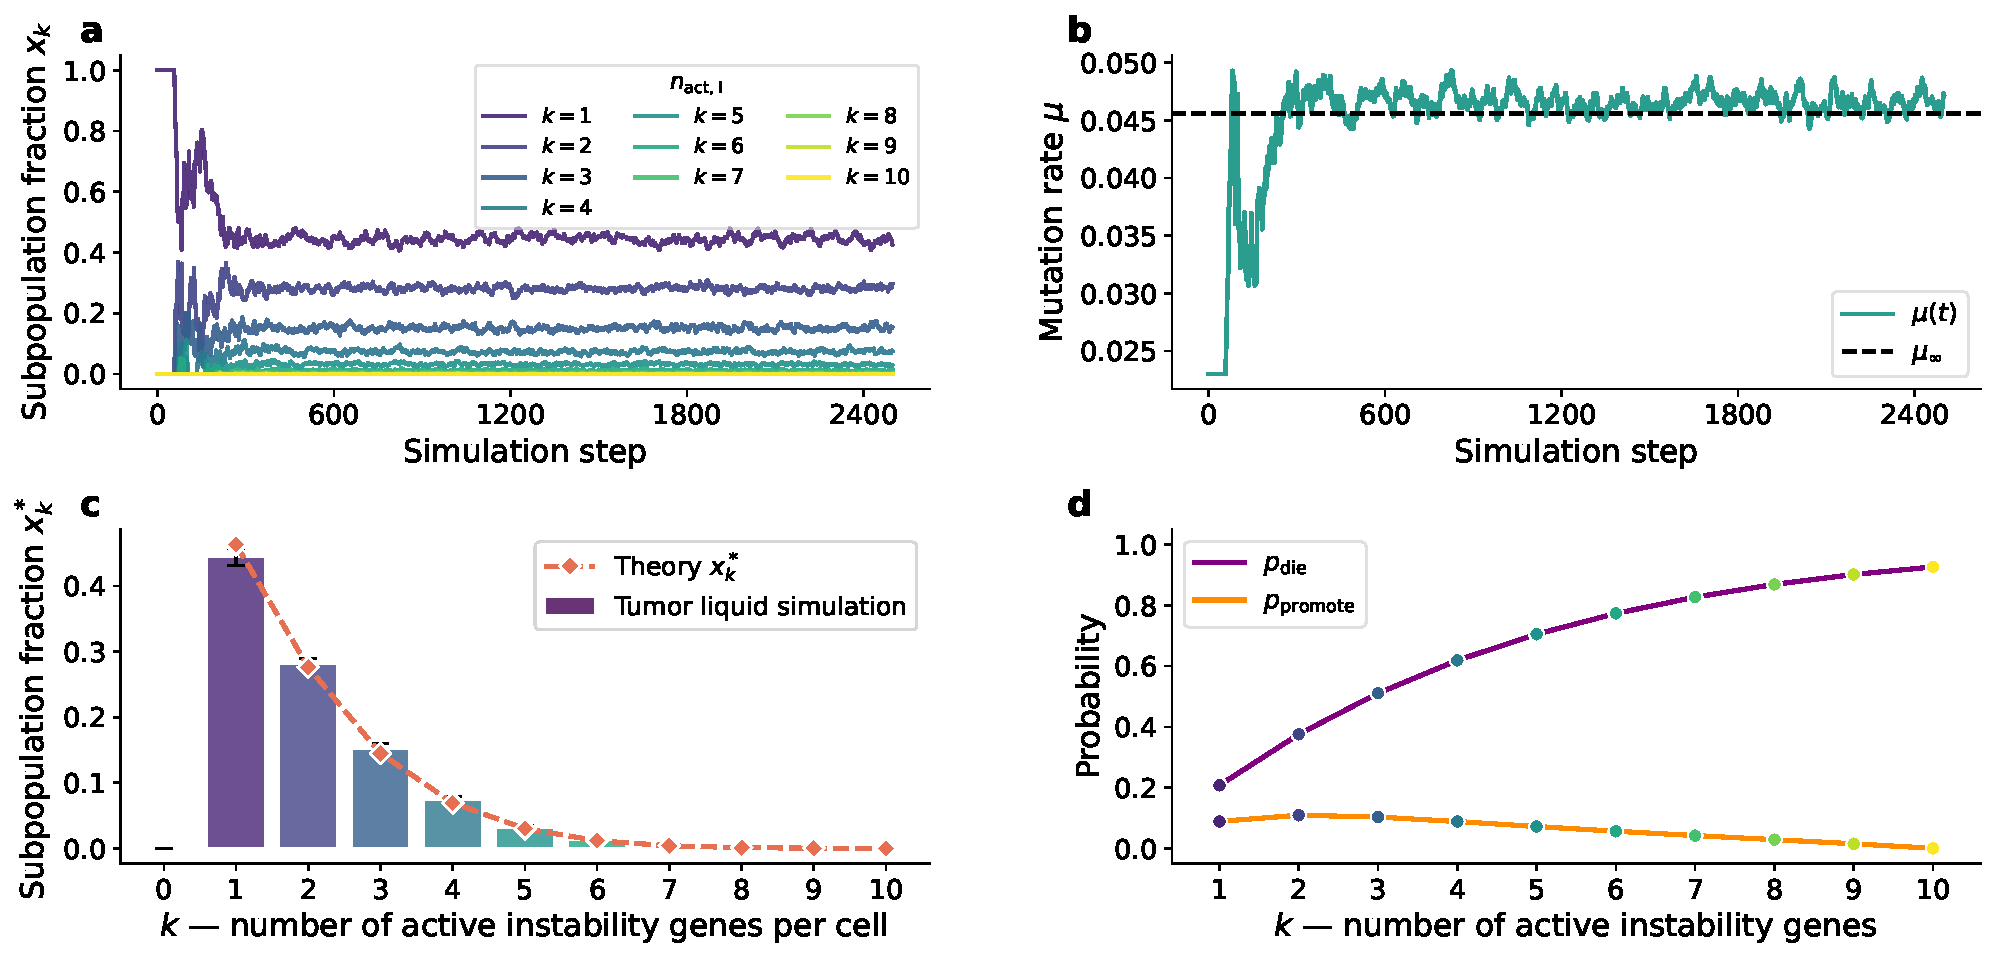
\includegraphics[width=\linewidth]{FigSM.pdf}
    \caption{Evolutionary dynamics and steady-state distribution of genetic instability in liquid tumor simulations. (a) Temporal evolution of subpopulation fractions $x_k$ as a function of simulation steps. The population is stratified by $k$, representing the number of active genetic instability genes per cell ($k \in [1, 10]$). Following initial transient fluctuations, the system relaxes into a stable, non-equilibrium steady state where subpopulations with low genomic instability ($k=1, 2, 3$) dominate the tumor mass. (b) Dynamic trajectory of the global mutation rate $\mu(t)$ (solid teal line) converging toward the theoretically predicted asymptotic limit $\mu_{\infty}$ (dashed black line). The rapid early expansion corresponds to a transient phase of mutational acceleration before stabilizing due to selective pressures. (c) Steady-state subpopulation fractions $f_k^*$ as a function of active instability genes. Simulated empirical distributions derived from the spatial tumor model (colored bars, error bars denote standard deviation across independent realizations) show excellent agreement with the analytical predictions derived from the mean-field framework (Eq.~\ref{eq:sta_distr}) (dashed orange line with diamonds, \texttt{Theory $x_k^*$}). (d) Functional dependence of phenotypic probabilities on the number of active instability genes $k$.}
    \label{fig:placeholder}
\end{figure}

\clearpage

\section{Mechanistic Internal-State Dynamics Across Karyotypic Regimes}
\label{sec:SM_karyotype}

To resolve the microscopic intracellular mechanisms driving the macroscopic expansion trajectories of Diploid ($D$, $dm = 0$), Whole-Chromosome Polyploid ($P$, $dm = 0.01$, whole-chromosome transfer), and Segmental Aneuploid ($A$, $dm = 0.01$, chunk-based transfer) tumors (Fig.~2e--f and Table~I in the main manuscript), we tracked the internal cellular state variables across 500-replicate solid-tumor ensembles (Fig.~\ref{fig:SM_karyotype_mechanisms}).

\subsection{Proliferation Saturation versus Effective Growth Propensity}
Under the Boolean OR dominance rule governing oncogenes ($\mathcal{O}$, Eq.~239), a single mutated allele at any present copy is sufficient to activate an oncogene locus. Moreover, because initial cancer seed cells start as diploid ($N_{\text{CHR}} = 2$) with zero active missegregation ($k_M = 0 \implies m = 0$), recessive inactivation of missegregation genes ($\mathcal{M}$, requiring homozygous hits on both homologues at rate $\sim \mu^2$) lags behind dominant oncogene activation (occurring at rate $\sim 2\mu$ per locus). Consequently, by the time chromosomal missegregation becomes active across the population, dominant oncogene mutations have already driven the intrinsic cellular division rate $\bar{r}(t)$ to its physiological ceiling $r_{\max} = 0.30$ across all three regimes (Fig.~\ref{fig:SM_karyotype_mechanisms}a, dashed curves). In fact, early chromosome gains slightly delay recessive tumor suppressor ($\mathcal{S}$) inactivation by increasing the number of wild-type alleles that must be mutated, and occasional chromosome losses in the mother cell can transiently strip a single-copy mutated oncogene, causing $\bar{r}(t)$ in $P$ and $A$ to lie marginally below $D$ during $t \in [250, 900]$.

Thus, karyotype-dependent growth differences are not driven by raw division speed, but rather by the \textbf{effective growth propensity} (Fig.~\ref{fig:SM_karyotype_mechanisms}a, solid curves):
\begin{equation}
    \bar{r}_{\mathrm{eff}}(t) = \bar{r}(t)\,\bigl(1 - \bar{p}_{\mathrm{d},\mathrm{tot}}(t)\bigr),
\end{equation}
which measures the net viable reproductive output per unit time after accounting for the total per-division death probability $\bar{p}_{\mathrm{d},\mathrm{tot}}(t)$.

\subsection{Decomposition of Per-Division Mortality: Redundancy Buffering versus Ploidy Ceiling}
During cell division, mortality arises from two distinct mechanistic pathways (Fig.~\ref{fig:SM_karyotype_mechanisms}b):
\begin{enumerate}
    \item \textbf{Essential Housekeeping ($\mathcal{H}$) Loss-of-Function ($\bar{p}_{\mathrm{d},\mathcal{H}}$, dashed curves):} A dividing lineage suffers essential gene failure if either (i) de novo point mutations simultaneously hit all remaining functional wild-type copies $k_{\mathrm{WT}}(t)$ at any of the $N_{\mathcal{H}} = 10$ essential loci, with probability
    \begin{equation}
        p_{\mathrm{d},\mathcal{H}}^{(\mathrm{mut})} = 1 - \bigl(1 - \mu^{k_{\mathrm{WT}}}\bigr)^{N_{\mathcal{H}}},
    \end{equation}
    or (ii) an asymmetric chromosomal or segmental loss (occurring with probability $m/2$ in the donor mother cell) strips the last remaining wild-type copy of a locus whose other $k - 1$ copies have already been mutated.
    \item \textbf{Hyperploid ($>5n$) and Nullisomic ($0n$) Allele-Threshold Violation ($\bar{p}_{\mathrm{d},\mathrm{ploidy}}$, dotted curves):} A missegregation event triggers immediate structural lethality if the recipient daughter exceeds the maximum viable copy number of $5$ alleles at any locus (or if the donor loses its sole remaining chromosome copy). In Whole-Chromosome Polyploidy ($P$), where all loci share a uniform copy number $N_{\text{CHR}}$, any missegregation in a cell at $N_{\text{CHR}} = 5$ pushes the daughter to $N_{\text{CHR}} = 6$, yielding $\bar{p}_{\mathrm{d},\mathrm{ploidy}}^{(P)} = m \bigl(f_{n_c=5} + f_{n_c=1}\bigr)$. In Segmental Aneuploidy ($A$), where the mean effective copy number per locus plateaus at an intermediate value ($\bar{k} \approx 3.76$ across $n_c = 5$ active slots), a random chromosomal fragment only breaches the $5$-copy cap if the severed segment overlaps a locus already present at $5$ copies, substantially reducing the boundary hazard ($\bar{p}_{\mathrm{d},\mathrm{ploidy}}^{(A)} \ll \bar{p}_{\mathrm{d},\mathrm{ploidy}}^{(P)}$).
\end{enumerate}

Combining these two contributions, $\bar{p}_{\mathrm{d},\mathrm{tot}} = 1 - (1 - \bar{p}_{\mathrm{d},\mathcal{H}})(1 - \bar{p}_{\mathrm{d},\mathrm{ploidy}})$, explains the three evolutionary regimes observed in the macroscopic tumor growth curves (Fig.~\ref{fig:SM_karyotype_mechanisms}a--b):
\begin{itemize}
    \item \textbf{Phase I --- Early Redundancy Buffering ($t \lesssim 750$):} Extra chromosome copies in $P$ and $A$ provide immediate allelic redundancy ($k_{\mathrm{WT}} > 2$), shielding cells from recessive $\mathcal{H}$ inactivation ($\bar{p}_{\mathrm{d},\mathcal{H}}(P) \le \bar{p}_{\mathrm{d},\mathcal{H}}(A) < \bar{p}_{\mathrm{d},\mathcal{H}}(D)$) before a significant fraction of the population reaches the $5n$ boundary. Consequently, $\bar{r}_{\mathrm{eff}}(P) \ge \bar{r}_{\mathrm{eff}}(A) > \bar{r}_{\mathrm{eff}}(D)$.
    \item \textbf{Phase II --- The $5n$ Ploidy Boundary Transition ($750 \lesssim t \lesssim 1450$):} Whole-chromosome gains rapidly drive the $P$ population against the $N_{\text{CHR}} = 5$ cap, causing $\bar{p}_{\mathrm{d},\mathrm{ploidy}}^{(P)}$ (brown dotted curve) to surge to $\approx 0.047$ per division. Because Segmental Aneuploidy ($A$, teal dotted curve) maintains an intermediate mean copy number ($\bar{k} \approx 3.76$), its $>5n$ boundary mortality remains more than fivefold lower ($\approx 0.009$), allowing $A$ to overtake $P$ ($\bar{r}_{\mathrm{eff}}(A) > \bar{r}_{\mathrm{eff}}(P) > \bar{r}_{\mathrm{eff}}(D)$) and establish the largest cumulative tumor mass.
    \item \textbf{Phase III --- Stationary Buffer Saturation ($t \gtrsim 1450$):} In the long-time limit, ongoing point mutations saturate the cryptic redundancy buffer across all karyotypes ($k_{\mathrm{WT}} \to 1$; Fig.~\ref{fig:SM_karyotype_mechanisms}c). Once viable cells retain only a single unmutated copy per essential gene, point-mutation mortality converges toward the same baseline across all regimes, while ongoing missegregation imposes a permanent mortality overhead ($\bar{p}_{\mathrm{d},\mathrm{ploidy}}$ plus chromosomal unmasking) on $P$ and $A$, yielding the asymptotic ordering $\bar{p}_{\mathrm{d},\mathrm{tot}}(D) < \bar{p}_{\mathrm{d},\mathrm{tot}}(A) < \bar{p}_{\mathrm{d},\mathrm{tot}}(P)$ and $\bar{r}_{\mathrm{eff}}(D) > \bar{r}_{\mathrm{eff}}(A) > \bar{r}_{\mathrm{eff}}(P)$.
\end{itemize}

\subsection{Cryptic Recessive Damage Accumulation and Buffer Erosion}
Figure~\ref{fig:SM_karyotype_mechanisms}c directly quantifies the internal genetic load buffered by multi-copy redundancy via the fraction of present essential housekeeping alleles that are mutated ($\mathrm{mut}_{\mathcal{H}}$) in surviving cells. Because complete inactivation of any essential locus is lethal, a viable cell with $k$ copies at an essential locus can harbor at most $k - 1$ mutated alleles. In Diploid ($D$) cells ($k = 2$), $\mathrm{mut}_{\mathcal{H}}$ is strictly bounded by the viability ceiling $(2 - 1)/2 = 0.50$ (black dotted line). By contrast, Whole-Chromosome Polyploid ($P$) and Segmental Aneuploid ($A$) cells survive while accumulating a massive cryptic reservoir of inactivated essential alleles, saturating at $(5 - 1)/5 = 0.80$ in $P$ and $\approx 0.76$ in $A$. Once this $(k - 1)/k$ redundancy buffer is completely filled, the protective survival advantage of polyploidy and aneuploidy is exhausted, converting chromosomal instability from an early adaptive buffer into a late-stage liability.

\begin{figure*}[htbp]
    \centering
    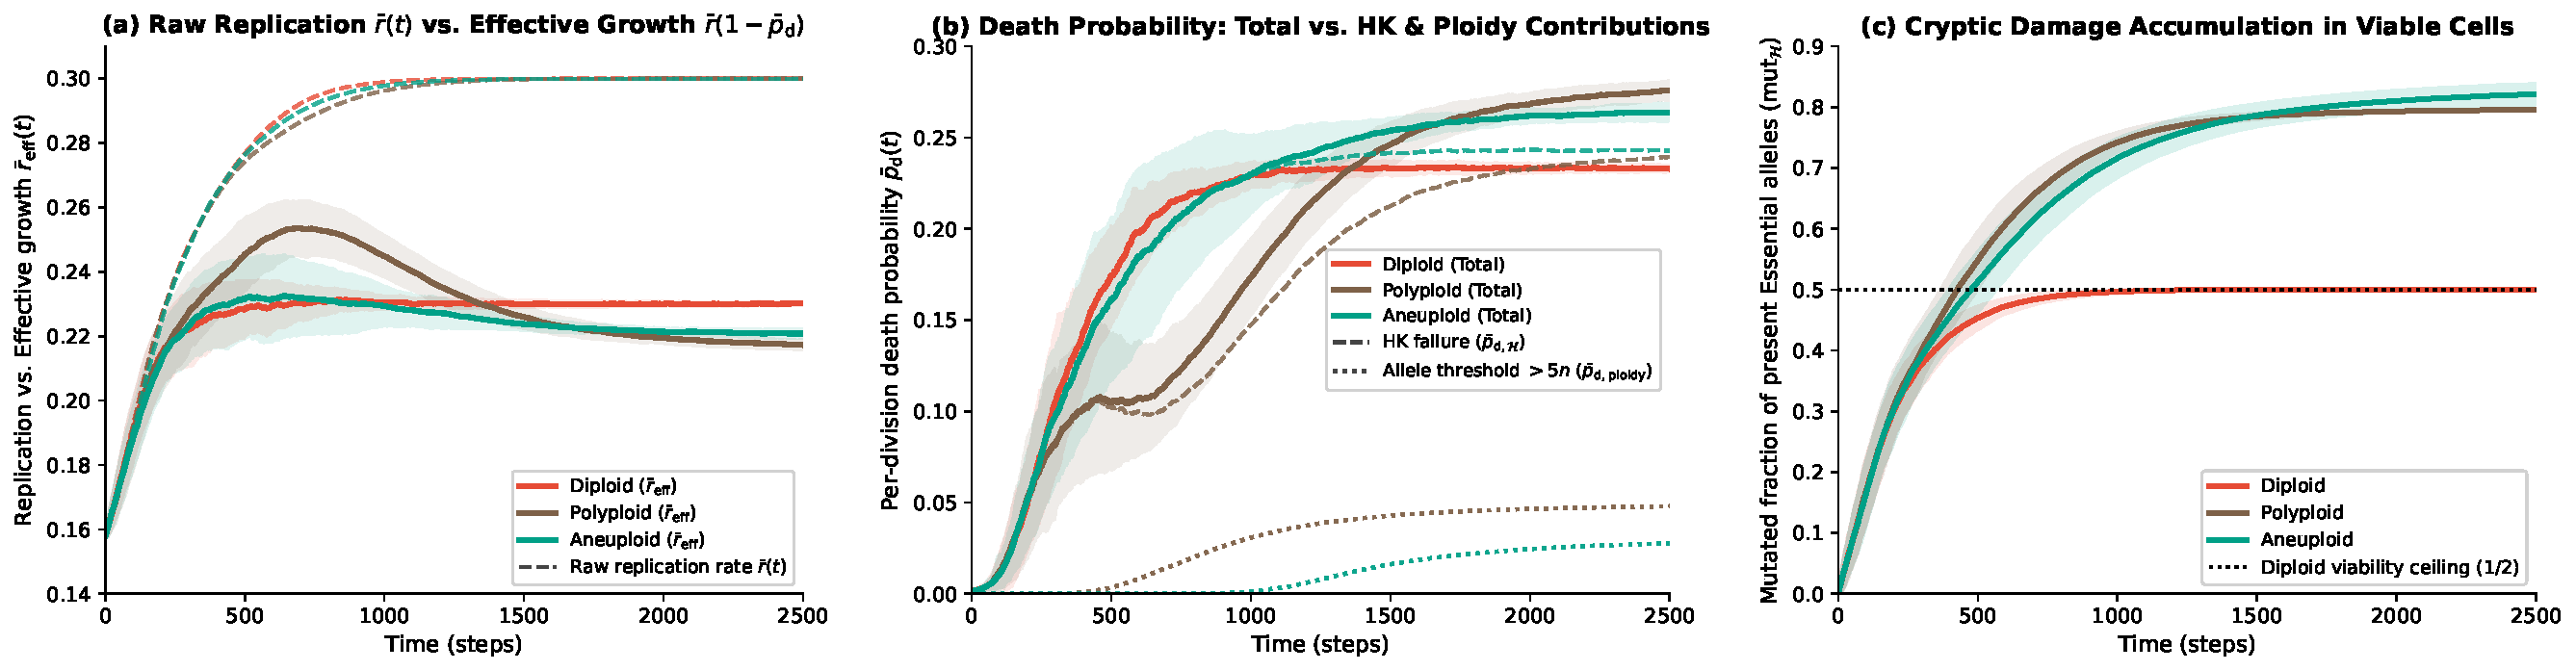
\includegraphics[width=\linewidth]{karyotype_mechanistic_internal_states.pdf}
    \caption{\textbf{Internal-state mechanistic dynamics across karyotypic regimes in solid tumors.}
    \textbf{(a)} Raw cellular replication rate $\bar{r}(t)$ (dashed curves) versus effective growth propensity $\bar{r}_{\mathrm{eff}}(t) = \bar{r}(t)(1 - \bar{p}_{\mathrm{d},\mathrm{tot}}(t))$ (solid curves). Because $\bar{r}(t)$ rapidly saturates at $r_{\max} = 0.30$ across all regimes, inter-karyotype growth differences are governed by differential cellular survival rather than intrinsic division speed.
    \textbf{(b)} Decomposition of the per-division death probability $\bar{p}_{\mathrm{d},\mathrm{tot}}(t)$ (solid curves) into essential housekeeping ($\mathcal{H}$) loss-of-function lethality ($\bar{p}_{\mathrm{d},\mathcal{H}}$, dashed curves) and hyperploid ($>5n$) allele-threshold lethality ($\bar{p}_{\mathrm{d},\mathrm{ploidy}}$, dotted curves).
    \textbf{(c)} Mutated fraction of present essential housekeeping alleles ($\mathrm{mut}_{\mathcal{H}}$) in surviving cells, demonstrating cryptic recessive damage accumulation above the diploid viability ceiling ($1/2 = 0.50$, black dotted line) up to the polyploid ($4/5 = 0.80$) and aneuploid ($\approx 0.76$) saturation limits. Curves and shaded bands denote ensemble means $\pm 1$ s.d.\ across surviving tumor realizations ($500$ replicates per regime).}
    \label{fig:SM_karyotype_mechanisms}
\end{figure*}

\end{document}



We collect every process that changes $C_k$, grouping by physical origin:

\paragraph{Term 1 --- Mother leaves class $k$ (loss).} The mother cell leaves class $k$ if she either promotes to any higher class $k+j$ or dies. This happens with total probability $1 - \alpha_k$, where $\alpha_k = P_{k \to k}$ is the faithful cloning probability:
\begin{equation}
    \text{(mother loss)} = -r_m\, f_k\, \phi_k\, (1 - \alpha_k)
\end{equation}

\paragraph{Term 2 --- Daughter clonal expansion (gain).} The daughter is placed on an available target (with effective probability $\phi_k$) and faithfully clones into class $k$ (probability $\alpha_k$). This combines rows 3 and 6 of Table~\ref{tab:transitions}:
\begin{equation}
    \text{(daughter clone)} = +r_m\, f_k\, \phi_k\, \alpha_k
\end{equation}
where $\phi_k = p_D + f_W \beta_{cw} + \sum_j f_j \beta_{cc}$ captures all possible successful placements.

\paragraph{Term 3 --- Cancer--cancer self-displacement (loss).} When a class-$k$ cell (call it cell~A) divides and its daughter targets \emph{another} class-$k$ cell (cell~B), cell~B is always removed. The daughter then undergoes mutation, leading to three possible outcomes:

\begin{enumerate}
    \item[\textbullet] Daughter clones faithfully ($\alpha_k$): cell~B is lost, but a new class-$k$ cell appears $\Rightarrow$ \textbf{net change = 0}.
    \item[\textbullet] Daughter promotes ($P_{k \to k+j}$): cell~B is lost, daughter enters class $k+j$ $\Rightarrow$ \textbf{net change = $-1$ for class $k$}.
    \item[\textbullet] Daughter dies ($\delta_k$): cell~B is lost, daughter dies $\Rightarrow$ \textbf{net change = $-1$ for class $k$}.
\end{enumerate}

In the ODE, this split is handled across two terms: Term~2 captures the gain from the first outcome (daughter clones, weighted by $\alpha_k$), while Term~3 captures the \emph{unconditional} loss of cell~B. Their net contribution is $r_m f_k^2 (\alpha_k - 1)/2 < 0$:
\begin{equation}
    \text{(self-displacement loss)} = -r_m\, \frac{f_k^2}{2}
\end{equation}

\paragraph{Term 4 --- Displacement by other cancer classes (loss).} Class-$k$ cells can be displaced by daughters from any other cancer class $j \neq k$:
\begin{equation}
    \text{(cross-class loss)} = -f_k \sum_{j \neq k} r_m\, f_j\, \beta_{cc}
\end{equation}

\paragraph{Term 5 --- Wild-type clearance (loss).} WT cells can divide and displace cancer class $k$ via Moran competition (row 9 of Table~\ref{tab:transitions}):
\begin{equation}
    \text{(WT clearance)} = -r_0\, f_W\, f_k\, \beta_{wc}
\end{equation}

\paragraph{Term 6 --- Promotion influx from all lower classes (gain).} Class $k$ receives cells from all classes $i < k$ through both mother and daughter promotions (transition probability $P_{i \to k}$). Since both occur only upon successful division:
\begin{equation}
    \text{(promotion influx)} = \sum_{i=1}^{k-1} 2\, r_m\, f_i\, \phi_i\, P_{i \to k}
\end{equation}
The factor $2$ reflects the dual source (mother + daughter) scaled by the division success probability $\phi_i$ and the multi-step promotion probability $P_{i \to k}$.



Here is an improved, publication-ready version of your text optimized for *PLOS Computational Biology*.

This draft enhances the rigorous, formal language required for a computational biology journal, standardizes the mathematical indices and variable notation ($N_{\mathcal{I}}$, $p_{\mu,i}$, and $\mu_{\infty}$), corrects the description of the transition matrix $\mathbf{A}$ (which is strictly **lower-bidiagonal**, not tridiagonal), resolves broken punctuation (like unclosed parentheses), and clarifies the biological rationale driving your asymptotic limits.

---

### Revised Text

The specific mutation rate around which the system stabilizes emerges naturally from intrinsic population dynamics shaped by evolutionary pressures. We focus our analysis on a regime where both the cellular replication rate and the mutational burden of housekeeping genes have reached saturation. This scenario occurs frequently within our framework due to the robust selective advantages associated with maximum proliferation and the accelerated early accumulation of housekeeping ($\mathcal{H}$) gene mutations.

At this stage, the tumor population can be conceptualized as a collection of distinct subpopulations, each defined by its number of phenotypically altered instability ($\mathcal{I}$) genes. Because a cell must possess at least one mutated $\mathcal{I}$ gene to be classified as malignant, the population can be partitioned into $N_{\mathcal{I}}$ discrete classes, denoted $x_1, \dots, x_{N_{\mathcal{I}}}$, where $x_i$ represents the fraction of cells harboring exactly $i$ mutated $\mathcal{I}$ genes. The sum over all subpopulation fractions is strictly conserved:
\begin{equation}
\sum_{i=1}^{N_{\mathcal{I}}} x_i = 1.
\end{equation}
Transitions between these subpopulations are driven by three primary microscopic processes: (i) *reproduction*, wherein a cell replicates and its daughter stochastically replaces another individual to satisfy a constant carrying capacity; (ii) *death*, resulting from lethal mutational hits to the remaining unmutated housekeeping ($\mathcal{H}$) alleles; and (iii) *mutation*, involving a novel hit to a functional $\mathcal{I}$ gene that pushes the cell into the next higher instability class.

Using a Master Equation approach, the temporal evolution of these subpopulation densities can be modeled as:
\begin{equation}
\begin{aligned}
\frac{dx_1}{dt} &= r x_1 \big(1 - p_{\mathrm{d},1} - p_{\mu,1}\big) - \Phi x_1, \[4pt]
\frac{dx_i}{dt} &= r x_i \big(1 - p_{\mathrm{d},i} - p_{\mu,i}\big) + r x_{i-1} p_{\mu,i-1} - \Phi x_i, \[4pt]
\frac{dx_{N_{\mathcal{I}}}}{dt} &= r x_{N_{\mathcal{I}}} \big(1 - p_{\mathrm{d},N_{\mathcal{I}}}\big) + r x_{N_{\mathcal{I}}-1} p_{\mu,N_{\mathcal{I}}-1} - \Phi x_{N_{\mathcal{I}}},
\end{aligned}
\label{eq:pop}
\end{equation}
where $2 \le i \le N_{\mathcal{I}}-1$. In a compact vector form, this system represents a standard discrete replicator-mutator equation:
\begin{equation}
\frac{d\mathbf{x}}{dt} = r \mathbf{A}\mathbf{x} - \Phi \mathbf{x},
\end{equation}
where $\mathbf{x} = (x_1, x_2, \ldots, x_{N_{\mathcal{I}}})^{\mathrm{T}}$ is the population state vector, $\Phi$ is a dynamic normalization factor (representing the average population fitness) that enforces a constant total tissue size, and $\mathbf{A}$ is a lower-bidiagonal transition matrix with the following structure:
\begin{widetext}

$$\mathbf{A} =
\begin{pmatrix}
1 - p_{\mathrm{d},1} - p_{\mu,1} & 0 & 0 & \cdots & 0 \\[4pt]
p_{\mu,1} & 1 - p_{\mathrm{d},2} - p_{\mu,2} & 0 & \cdots & 0 \\[4pt]
0 & p_{\mu,2} & 1 - p_{\mathrm{d},3} - p_{\mu,3} & \cdots & 0 \\[4pt]
\vdots & \vdots & \vdots & \ddots & \vdots \\[4pt]
0 & 0 & 0 & p_{\mu,N_{\mathcal{I}}-1} & 1 - p_{\mathrm{d},N_{\mathcal{I}}}
\end{pmatrix}.$$

\end{widetext}
Within this matrix, the class-dependent death probability $p_{\text{d},1}$ is defined as:
\begin{equation}
p_{\text{d},i} = 1 - (1 - i \cdot \Delta\mu)^{N_{\mathcal{H}}}.
\end{equation.
To calculate the forward transition probability $p_{\mu,i}$ between successive instability classes, we consider a limiting case where each instability gene carries at most one unmutated allele. This configuration represents the asymptotic state of the system because the accumulation of mutations eventually saturates the underlying phenotype due to the AND-gate logic governing the gene classes. In this limiting case, the forward mutation probability from class $i$ to class $i+1$ scales as:
\begin{equation}
p_{\mu,i} = 1 - (1 - i \cdot \Delta\mu)^{(N_{\mathcal{I}} - i)}.
\end{equation}
Because back-mutations are omitted and simultaneous multi-step jumps are neglected as higher-order effects, transitions are strictly unidirectional. The resulting probabilities for a representative $10$-population model are reported in Fig.~\ref{fig:pop_dyn}d.

From this analytical framework, it is possible to compute the stationary concentration for each malignant subpopulation (see Materials and Methods for the full derivation), which can then be directly validated against findings from long-term stochastic simulations. Fig.~\ref{fig:pop_dyn}a demonstrates that the simulated system successfully converges to a stable distribution of subpopulation densities, matching the theoretical predictions with high fidelity (Fig.~\ref{fig:pop_dyn}c). Furthermore, as illustrated in Fig.~\ref{fig:pop_dyn}b, the long-term, population-averaged mutation rate across the tissue fluctuates stably around the predicted asymptotic value $\mu_{\infty}$. This quantitative alignment highlights the predictive reproducibility of our analytical reduction and supports the conclusion that the linear growth phases observed in simulations correspond to stable, ecological-like equilibria among competing clonal subpopulations under conditions of growth-rate and housekeeping saturation.

Crucially, this emergent equilibrium state does not coincide with the boundary between tumor proliferation and extinction; rather, it acts as a stable dynamical attractor deep within the viable phase space. In contrast, the phase transition line—governed by the exact threshold where replication forces balance mutation-induced cell death—remains critical in determining whether the neoplastic population can escape early stochastic reabsorption and establish this linear growth phase in the first place.

Finally, this framework provides an explicit explanation for why some tumors, despite temporarily settling into a stable mutational state, are driven to delayed extinction if they cross above the phase transition line. Because mutation transitions are strictly unidirectional, if stochastic fluctuations or intense selective sweeps cause the absolute loss of all cells in the lowest mutational classes, the tumor cannot regenerate them. Consequently, the lower boundary of the matrix shifts, making the lowest active class $x_j$ instead of $x_1$. This truncation forces a permanent upward shift in the baseline mutation rate across the entire remaining tumor population, escalating the mutational burden and driving the system into an irreversible shrinking phase.

---

### Key Refinements Explained:

1. **Mathematical Nomenclature (Matrix Structure):** The original text characterized matrix $\mathbf{A}$ as a *"tridiagonal structure"*. However, because there are no non-zero entries above the main diagonal (due to the absence of back-mutations), it is strictly a **lower-bidiagonal matrix**. Correcting this ensures it passes strict mathematical review.
2. **Variable & Index Standardization:** * Unified your indices across equations: changed text references from $N_I$ to $N_{\mathcal{I}}$ and standardized $p_{\text{mut},i}$ to $p_{\mu,i}$ to preserve exact symmetry with the text inside your systems of differential equations.
* Clarified a critical indexing typo in the definition of forward transition: changed *"from class $\mathcal{I}$ to $i+1$"* to *"from class $i$ to class $i+1$"*.
* Cleaned up minor formatting artifacts like unclosed parenthetical punctuation (e.g., `2 \le i \le N_\mathcal{I}-1)`` $\rightarrow$ `2 \le i \le N_{\mathcal{I}}-1`and`\mu_{\infty})`$\rightarrow$`\mu_{\infty}`).


3. **Elevated Academic Presentation:** * Replaced casual phrasing like *"this is a case in which the system eventually will end up in the long run"* with *"This configuration represents the asymptotic state of the system..."*
* Refine sentence transitions: Changed *"In panel b, moreover, it is shown"* to *"Furthermore, as illustrated in Fig.~\ref{fig:pop_dyn}b..."* to achieve the authoritative, passive voice favored in physical and computational biology literature.